\begin{figure}
    \centering
    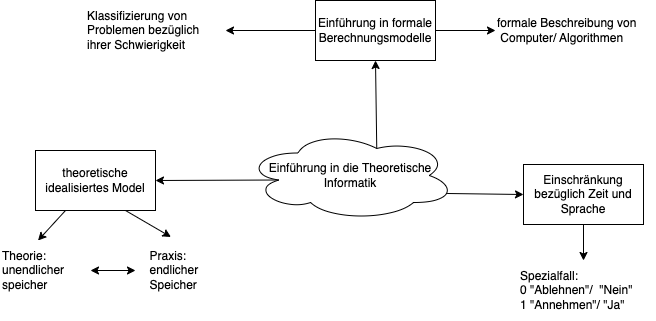
\includegraphics[width=1\textwidth]{Grundlagen/svg_files/Einführung.png}
    \caption{Überblick theoretische Informatik}
    \label{fig:example}
\end{figure}
\mysection{Grundlagen}
\mysubsection{Notationen und begriffe}
\begin{itemize}
    \item \(\mathbb{N}\) bezeichnet die \{1, 2, 3\}
    \item \(\mathbb{N}_{0}\), sei \([n]\) = \{1,\(\ldots \),n\} und \([n]_{0}\) = \{0, 1, \(\ldots \),n\} 
    \item Für eine Menge A und \(n \in \mathbb{N}\) ist \(A^{n} = \{(a_{1},\ldots, a_{n}): a_{1}, \ldots a_{n}\in A\}\)
    \item Für n \(\in \mathbb{N}\) ist eine n-äre partielle funktion \(\varphi : A^{n} \leadsto B \) eine Funktion mit dom\((\varphi) \supseteq A^{n}\) und Im\((\varphi) \subseteq B.\) 
    Für \(a_{1}, ..., a_{n} \in A\) bedeuted \(\varphi(a_{1}, ..., a_{n})\downarrow\), dass (\(a_{1}, ..., a_{n})\in \text{dom}(\varphi)\) gilt und \(\varphi(a_{1}, ..., a_{n})\uparrow \)bedeutet, 
    dass (\(a_{1}, ..., a_{n}) \notin \text{dom}(\varphi)\). Statt \(\varphi(a_{1}, ..., a_{n})\uparrow\) schreiben wir auch \(\varphi(a_{1}, ..., a_{n}) = \uparrow\).
    Die partielle Funktion \(\varphi\) ist total, wenn dom(\(\varphi) = A^{n}\) gilt.
    \item Eine lineare Ordnung, auch totale Ordnung, auf einer Menge A ist eine Relation \(\leq  \subseteq  A^{n}\) m sodass die folgende Eigenschaften erfüllt sind. 
    (wie für Relationen üblich verwenden wir hier Infixntation, schreiben also für a,b \(\in\) A den Ausdruck a \(\leq\)  b anstatt (a,b) \(\in \leq\)): 
    \begin{enumerate}
        \item[(i)] \(a \leq  a \forall a \in A\) (Reflexivität)
        \item[(ii)]\( a \leq  b  \land  b \leq  a \Rightarrow  a = b \forall a,b \in A\) (Antisymetrie)
        \item[(iii)] \(a \leq  b, b \leq  c \Rightarrow a \leq  c foralla,b,c \in A\) (Transitiität)
        \item[(iv)] \(a \leq  b \vee b \leq  a \forall a,b \in A\) (Totalität)
    \end{enumerate} 
\end{itemize}

\mysubsection{Alphabet, Wörter und Sprachen}
    Eingaben und Ausgaben in unseren Berechnungsmodellen werden wörter genannt, wobei wir beliebige Zeichenketten als Wörter zulassen.

\mysubsubsection{Definition (Alphabet)}
    Ein Alphabet ist eine nichtleere endliche Menge \(\Sigma\). Das Alphabet \(\Sigma\) wird \(\lvert \Sigma \rvert\)- är bezeichnet. Die Elemente von \(\Sigma\) heißen Buchstaben oder Symbole.

\mysubsubsection{Definition (Wörter)}
    Ein Wort über einem Alphabet \(\Sigma\) ist eine endliche Folge von Symbolen aus \(\Sigma\). Die Länge eines Wortes w ist \(\lvert w \rvert\). Für \(i \in\lvert w \rvert\) bezeichnet w(i) das i-te Element von w und für Symbole \(a_{1}, \cdots, a_{n} \in \Sigma\) bezeichnet \(a_{1}, \cdots, a_{n}\) das Wort w der Länge n mit \(w(i) = a_{i} \forall i\in [n]\). Das Wort der Länge 0 heißt leeres Wort und wird \(\lambda\) bezeichnet. Ein Wort der länge 1 wird mit dem Symbol w(1) identifiziert.

\mysubsubsection{Definition (Binäraphabet, Binärwörter)}
    Das Alphabet \{0, 1\} heißt Binäralphabet. Die Wörter über dem Binäralphabet heißen Binärwörter.

\mysubsubsection{Sprache}
    Eine \textbf{Sprache} ist eine Menge von Wörter über einem gemeinsahmen Alphabet \(\Sigma\). Einige einfache grundlegenden Sprachen sind die folgenden.

\mysubsubsection{Definition}
    Die Menge Aller Wörter über \(\Sigma\) wird mit \(\Sigma^{*}\) bezeichnet. Für \(n \in \mathbb{N}_{0}\) setzen wir:
    \begin{itemize}
        \item[] \(\Sigma^{\leq n} := \{w \in \Sigma^{*} : \lvert w \rvert \leq n\}\)
        \item[] \(\Sigma^{=n} := \{w \in \Sigma^{*} : \lvert w \rvert = n\}\)
        \item[] \(\Sigma^{\geq n} := \{w \in \Sigma^{*} : \lvert w \rvert \geq n\}\)
        \item[] \(\Sigma^{+} := \Sigma^{\leq 1}\)
    \end{itemize}

\mysubsubsection{Definition (Verkettung)}
    Für Wörter \(w_{1}, w_{2}\) ist die verkettung  \(w_{1} \circ w_{2}\), auch \(w_{1}w_{2}\), von \(w_{1}\) und \(w_{2}\) ist definiert durch:
    \[
        w_{1} \circ w_{2} := w_{1} \cdots w_{1} (\lvert w_{1} \rvert)w_{2} \cdots w_{2} (\lvert w_{2} \rvert)
    \]
    Für ein Wort w und \(n \in \mathbb{N}_{0}\) ist \(w^{k}\) induktiv definiert durch \(w^{n} := \lambda \) falls n = 0 und \(w^{n} := w^{n-1} \circ w^{n} \)falls \(n \geq  1\). Für eine Sprachen\( L_{1}, L_{2}\) sei durch \(L_{1} \circ L_{1}, \)auch \(L_{1}L_{2}\) definiert durch
    \[
        L_{1} \circ L_{1} := \{w_{1}w_{2} : w_{1} \in L_{1}, w_{2} \in L_{2}\}
    \]
    Für eine Sprache L und und \(n \in\mathbb{N}_{0}\) ist \(L^{n}\) moduliert definiert durch \(L^{n} = \{\lambda\} \)falls n = 0 und \(L^{n} := L \cdot L^{n - 1}\) falls \(n \geq 1\). Zudem sei \(L^{*} := \bigcup \limits_{n \in \mathbb{N}_{0}}L^{n}\). Für ein Wort w und eine Sprache L sei \(wL :=\{w\}\circ\) und \(Lw := L\circ \{w\}\).\\Wir folgen der Konventrion, dass \(\bullet^{n}\) und \(\bullet^{*}\) stärker binden als 0;?? für Wörter u, v gilt also \(uv = u \circ (v^{n})\). Insbesondere gilt auch \(ab^{n} = a(b^{n})\) für Symbole a, b eines Alphabets \(\Sigma\).

    \mysubsubsection{Definition (Präfix, Infix, Suffix)}
    Seiene u, v Wörter.
    \begin{itemize}
        \item [(i)] u ist Präfix von v, kurz u \(\sqsubseteq\) v, falls es ein Wort w gibt ,sodass uw = v.
        \item [(ii)] u ist Infix von v falls es Wörter \(w_{1}, w_{1}\) gibt sodass \(v = w_{1} u w_{2}\)
        \item [(iii)] u ist Suffic von v, falls es ein Wort w gibt, sodass v = wu.
    \end{itemize}

\mysubsubsection{Definition (präfixfrei)}
    Eine Sprache heißt \textbf{präfixfrei}, wenn \(u\sqsubseteq v \Rightarrow u = v \forall u,v \in L\).

\mysubsubsection{Definition (Homomorphismus)}
    Für Sprache L und M heißt eine Funktion \(\varphi : L \rightarrow M\) \textbf{Homomorphismus von Sprachen}, wenn \(\varphi(uv) = \varphi (u) \varphi (v) \forall u, v \in L\) gilt.

\mysubsubsection{Definition (Längenlexikographische Ordnung)} 
    Ist \(\Sigma\) ein Alphabet und \(\leq\)  eine lineare Ordnung auf \(\Sigma\), so ist die zu \(\leq\)  gehörige \textbf{längenlexikographische Ordnung} \(\leq_{llex}\) auf \(\Sigma^{*}\) die lineare Ordnung für die \(u \leq_{llex} v\) genau dann für zwei verschiedene \(u, v\in \Sigma^{*} \)gilt, wenn eine der folgenden Bedingungen gilt:
\begin{itemize}
    \item \(\lvert u \rvert < \lvert v \rvert\)
    \item \(\lvert u \rvert = \lvert v \rvert\) und ist \(i \in [|u|]\) minimal mit 
    \(u(i) \neq v(i)m so gilt u(i) \leq v(i)\).
\end{itemize}
\textbf{Bemerkung: }Oft gehen wir von einer impliziten Ordnung auf \(\Sigma\) aus. Ist \(\Sigma = {a_{1}, \cdots, a_{n}}\) so gilt\( a_{1}\leq \cdots \leq a_{n}
\)
\mysubsubsection{Bemerkung} 
    Sei \(\Sigma\) ein Alphabet \(\forall w \in \Sigma^{*}\) ist \({v\in \Sigma^{*} : v \leq_{llex}w}\) endlich. Dies erlaubt es uns für ein Alphabet \(\Sigma\) die Wörter über \(\Sigma\) in längenlexilographischen Reihenfolge \(w_{1}, w_{2}, \cdots\) zu betrachten, wobei wir \(w_{i}\) für \(i \in \mathbb{N}\) als kleinstes Element von \(\Sigma^{*}/{w_{1},\cdots, w_{i-1}}\) gewählt sei. Wir identifizieren oft \(\mathbb{N}_{0} mit {0, 1}^{*}\) indem wir \(i \in \mathbb{N}_{0}\) mit in die längenlexilographische Reihenfolge (i+1)-ten Wort\( w_{i+1} \in {0,1}^{*} \)identifiziernen.
    \begin{center}
        \begin{tabular}{ c c c c c }
            \(\mathbb{N}_{0}\) & 0 & 1 & 2 & 3\\ 
            \(\{0, 1\}^{*}\) & \(\lambda\) & 0 & 1 & 00\\
        \end{tabular}
    \end{center}

\mysubsubsection{Definition}
    Es bezeichnet bin : \(\mathbb{N}_{0} \rightarrow \{0, 1\}^{*}\) die Funktion, für die bin(i) das in längenlexikographischer Reihenfolge (i+1)-te Binärwort ist \(\forall i \in \mathbb{N}_{0}\)

\mysubsubsection{Bemerkung}
    \(\forall i \in \mathbb{N}_{0}\) ist 1 bin(i) die Binärdarstellung von i+1. Umgekehrt ist \(\forall w \in {0, 1}^{*}\) das \((2^{|w|} + \underset{i \in [|w|]}{\Sigma} w(i) 2^{|w|-i})\)-te Binärwort.
